\documentclass[12pt]{article}
\usepackage{graphicx}
\usepackage{bbm}
%packages
%\usepackage{latexsym}
\usepackage{graphicx}
\usepackage{color}
\usepackage{amsmath}
\usepackage{dsfont}
\usepackage{placeins}
\usepackage{amssymb}
\usepackage{wasysym}
\usepackage{abstract}
\usepackage{hyperref}
\usepackage{etoolbox}
\usepackage{datetime}
\usepackage{xcolor}
\usepackage{alphalph}
\settimeformat{ampmtime}

%\usepackage{pstricks,pst-node,pst-tree}

%\usepackage{algpseudocode}
%\usepackage{amsthm}
%\usepackage{hyperref}
%\usepackage{mathrsfs}
%\usepackage{amsfonts}
%\usepackage{bbding}
%\usepackage{listings}
%\usepackage{appendix}
\usepackage[margin=1in]{geometry}
%\geometry{papersize={8.5in,11in},total={6.5in,9in}}
%\usepackage{cancel}
%\usepackage{algorithmic, algorithm}

\makeatletter
\def\maxwidth{ %
  \ifdim\Gin@nat@width>\linewidth
    \linewidth
  \else
    \Gin@nat@width
  \fi
}
\makeatother

\definecolor{fgcolor}{rgb}{0.345, 0.345, 0.345}
\newcommand{\hlnum}[1]{\textcolor[rgb]{0.686,0.059,0.569}{#1}}%
\newcommand{\hlstr}[1]{\textcolor[rgb]{0.192,0.494,0.8}{#1}}%
\newcommand{\hlcom}[1]{\textcolor[rgb]{0.678,0.584,0.686}{\textit{#1}}}%
\newcommand{\hlopt}[1]{\textcolor[rgb]{0,0,0}{#1}}%
\newcommand{\hlstd}[1]{\textcolor[rgb]{0.345,0.345,0.345}{#1}}%
\newcommand{\hlkwa}[1]{\textcolor[rgb]{0.161,0.373,0.58}{\textbf{#1}}}%
\newcommand{\hlkwb}[1]{\textcolor[rgb]{0.69,0.353,0.396}{#1}}%
\newcommand{\hlkwc}[1]{\textcolor[rgb]{0.333,0.667,0.333}{#1}}%
\newcommand{\hlkwd}[1]{\textcolor[rgb]{0.737,0.353,0.396}{\textbf{#1}}}%

\usepackage{framed}
\makeatletter
\newenvironment{kframe}{%
 \def\at@end@of@kframe{}%
 \ifinner\ifhmode%
  \def\at@end@of@kframe{\end{minipage}}%
  \begin{minipage}{\columnwidth}%
 \fi\fi%
 \def\FrameCommand##1{\hskip\@totalleftmargin \hskip-\fboxsep
 \colorbox{shadecolor}{##1}\hskip-\fboxsep
     % There is no \\@totalrightmargin, so:
     \hskip-\linewidth \hskip-\@totalleftmargin \hskip\columnwidth}%
 \MakeFramed {\advance\hsize-\width
   \@totalleftmargin\z@ \linewidth\hsize
   \@setminipage}}%
 {\par\unskip\endMakeFramed%
 \at@end@of@kframe}
\makeatother

\definecolor{shadecolor}{rgb}{.77, .77, .77}
\definecolor{messagecolor}{rgb}{0, 0, 0}
\definecolor{warningcolor}{rgb}{1, 0, 1}
\definecolor{errorcolor}{rgb}{1, 0, 0}
\newenvironment{knitrout}{}{} % an empty environment to be redefined in TeX

\usepackage{alltt}
\usepackage[T1]{fontenc}

\newcommand{\qu}[1]{``#1''}
\newcounter{probnum}
\setcounter{probnum}{1}

%create definition to allow local margin changes
\def\changemargin#1#2{\list{}{\rightmargin#2\leftmargin#1}\item[]}
\let\endchangemargin=\endlist 

%allow equations to span multiple pages
\allowdisplaybreaks

%define colors and color typesetting conveniences
\definecolor{gray}{rgb}{0.5,0.5,0.5}
\definecolor{black}{rgb}{0,0,0}
\definecolor{white}{rgb}{1,1,1}
\definecolor{blue}{rgb}{0.5,0.5,1}
\newcommand{\inblue}[1]{\color{blue}#1 \color{black}}
\definecolor{green}{rgb}{0.133,0.545,0.133}
\newcommand{\ingreen}[1]{\color{green}#1 \color{black}}
\definecolor{yellow}{rgb}{1,1,0}
\newcommand{\inyellow}[1]{\color{yellow}#1 \color{black}}
\definecolor{orange}{rgb}{0.9,0.649,0}
\newcommand{\inorange}[1]{\color{orange}#1 \color{black}}
\definecolor{red}{rgb}{1,0.133,0.133}
\newcommand{\inred}[1]{\color{red}#1 \color{black}}
\definecolor{purple}{rgb}{0.58,0,0.827}
\newcommand{\inpurple}[1]{\color{purple}#1 \color{black}}
\definecolor{backgcode}{rgb}{0.97,0.97,0.8}
\definecolor{Brown}{cmyk}{0,0.81,1,0.60}
\definecolor{OliveGreen}{cmyk}{0.64,0,0.95,0.40}
\definecolor{CadetBlue}{cmyk}{0.62,0.57,0.23,0}

%define new math operators
\DeclareMathOperator*{\argmax}{arg\,max~}
\DeclareMathOperator*{\argmin}{arg\,min~}
\DeclareMathOperator*{\argsup}{arg\,sup~}
\DeclareMathOperator*{\arginf}{arg\,inf~}
\DeclareMathOperator*{\convolution}{\text{\Huge{$\ast$}}}
\newcommand{\infconv}[2]{\convolution^\infty_{#1 = 1} #2}
%true functions

%%%% GENERAL SHORTCUTS

%shortcuts for pure typesetting conveniences
\newcommand{\bv}[1]{\boldsymbol{#1}}

%shortcuts for compound constants
\newcommand{\BetaDistrConst}{\dfrac{\Gamma(\alpha + \beta)}{\Gamma(\alpha)\Gamma(\beta)}}
\newcommand{\NormDistrConst}{\dfrac{1}{\sqrt{2\pi\sigma^2}}}

%shortcuts for conventional symbols
\newcommand{\tsq}{\tau^2}
\newcommand{\tsqh}{\hat{\tau}^2}
\newcommand{\sigsq}{\sigma^2}
\newcommand{\sigsqsq}{\parens{\sigma^2}^2}
\newcommand{\sigsqovern}{\dfrac{\sigsq}{n}}
\newcommand{\tausq}{\tau^2}
\newcommand{\tausqalpha}{\tau^2_\alpha}
\newcommand{\tausqbeta}{\tau^2_\beta}
\newcommand{\tausqsigma}{\tau^2_\sigma}
\newcommand{\betasq}{\beta^2}
\newcommand{\sigsqvec}{\bv{\sigma}^2}
\newcommand{\sigsqhat}{\hat{\sigma}^2}
\newcommand{\sigsqhatmlebayes}{\sigsqhat_{\text{Bayes, MLE}}}
\newcommand{\sigsqhatmle}[1]{\sigsqhat_{#1, \text{MLE}}}
\newcommand{\bSigma}{\bv{\Sigma}}
\newcommand{\bSigmainv}{\bSigma^{-1}}
\newcommand{\thetavec}{\bv{\theta}}
\newcommand{\thetahat}{\hat{\theta}}
\newcommand{\thetahatmle}{\hat{\theta}_{\mathrm{MLE}}}
\newcommand{\thetavechatmle}{\hat{\thetavec}_{\mathrm{MLE}}}
\newcommand{\muhat}{\hat{\mu}}
\newcommand{\musq}{\mu^2}
\newcommand{\muvec}{\bv{\mu}}
\newcommand{\muhatmle}{\muhat_{\text{MLE}}}
\newcommand{\lambdahat}{\hat{\lambda}}
\newcommand{\lambdahatmle}{\lambdahat_{\text{MLE}}}
\newcommand{\etavec}{\bv{\eta}}
\newcommand{\alphavec}{\bv{\alpha}}
\newcommand{\minimaxdec}{\delta^*_{\mathrm{mm}}}
\newcommand{\ybar}{\bar{y}}
\newcommand{\xbar}{\bar{x}}
\newcommand{\Xbar}{\bar{X}}
\newcommand{\phat}{\hat{p}}
\newcommand{\Phat}{\hat{P}}
\newcommand{\Zbar}{\bar{Z}}
\newcommand{\iid}{~{\buildrel iid \over \sim}~}
\newcommand{\inddist}{~{\buildrel ind \over \sim}~}
\newcommand{\approxdist}{~{\buildrel approx \over \sim}~}
\newcommand{\equalsindist}{~{\buildrel d \over =}~}
\newcommand{\loglik}[1]{\ell\parens{#1}}
\newcommand{\thetahatkminone}{\thetahat^{(k-1)}}
\newcommand{\thetahatkplusone}{\thetahat^{(k+1)}}
\newcommand{\thetahatk}{\thetahat^{(k)}}
\newcommand{\half}{\frac{1}{2}}
\newcommand{\third}{\frac{1}{3}}
\newcommand{\twothirds}{\frac{2}{3}}
\newcommand{\fourth}{\frac{1}{4}}
\newcommand{\fifth}{\frac{1}{5}}
\newcommand{\sixth}{\frac{1}{6}}

%shortcuts for vector and matrix notation
\newcommand{\A}{\bv{A}}
\newcommand{\At}{\A^T}
\newcommand{\Ainv}{\inverse{\A}}
\newcommand{\B}{\bv{B}}
\newcommand{\K}{\bv{K}}
\newcommand{\Kt}{\K^T}
\newcommand{\Kinv}{\inverse{K}}
\newcommand{\Kinvt}{(\Kinv)^T}
\newcommand{\M}{\bv{M}}
\newcommand{\Bt}{\B^T}
\newcommand{\Q}{\bv{Q}}
\newcommand{\Qt}{\Q^T}
\newcommand{\R}{\bv{R}}
\newcommand{\Rt}{\R^T}
\newcommand{\Z}{\bv{Z}}
\newcommand{\X}{\bv{X}}
\newcommand{\Xsub}{\X_{\text{(sub)}}}
\newcommand{\Xsubadj}{\X_{\text{(sub,adj)}}}
\newcommand{\I}{\bv{I}}
\newcommand{\Y}{\bv{Y}}
\newcommand{\sigsqI}{\sigsq\I}
\renewcommand{\P}{\bv{P}}
\newcommand{\Psub}{\P_{\text{(sub)}}}
\newcommand{\Pt}{\P^T}
\newcommand{\Pii}{P_{ii}}
\newcommand{\Pij}{P_{ij}}
\newcommand{\IminP}{(\I-\P)}
\newcommand{\Xt}{\bv{X}^T}
\newcommand{\XtX}{\Xt\X}
\newcommand{\XtXinv}{\parens{\Xt\X}^{-1}}
\newcommand{\XtXinvXt}{\XtXinv\Xt}
\newcommand{\XXtXinvXt}{\X\XtXinvXt}
\newcommand{\x}{\bv{x}}
\newcommand{\onevec}{\bv{1}}
\newcommand{\oneton}{1, \ldots, n}
\newcommand{\yoneton}{y_1, \ldots, y_n}
\newcommand{\yonetonorder}{y_{(1)}, \ldots, y_{(n)}}
\newcommand{\Yoneton}{Y_1, \ldots, Y_n}
\newcommand{\iinoneton}{i \in \braces{\oneton}}
\newcommand{\onetom}{1, \ldots, m}
\newcommand{\jinonetom}{j \in \braces{\onetom}}
\newcommand{\xoneton}{x_1, \ldots, x_n}
\newcommand{\Xoneton}{X_1, \ldots, X_n}
\newcommand{\xt}{\x^T}
\newcommand{\y}{\bv{y}}
\newcommand{\yt}{\y^T}
\renewcommand{\c}{\bv{c}}
\newcommand{\ct}{\c^T}
\newcommand{\tstar}{\bv{t}^*}
\renewcommand{\u}{\bv{u}}
\renewcommand{\v}{\bv{v}}
\renewcommand{\a}{\bv{a}}
\newcommand{\s}{\bv{s}}
\newcommand{\yadj}{\y_{\text{(adj)}}}
\newcommand{\xjadj}{\x_{j\text{(adj)}}}
\newcommand{\xjadjM}{\x_{j \perp M}}
\newcommand{\yhat}{\hat{\y}}
\newcommand{\yhatsub}{\yhat_{\text{(sub)}}}
\newcommand{\yhatstar}{\yhat^*}
\newcommand{\yhatstarnew}{\yhatstar_{\text{new}}}
\newcommand{\z}{\bv{z}}
\newcommand{\zt}{\z^T}
\newcommand{\bb}{\bv{b}}
\newcommand{\bbt}{\bb^T}
\newcommand{\bbeta}{\bv{\beta}}
\newcommand{\beps}{\bv{\epsilon}}
\newcommand{\bepst}{\beps^T}
\newcommand{\e}{\bv{e}}
\newcommand{\Mofy}{\M(\y)}
\newcommand{\KofAlpha}{K(\alpha)}
\newcommand{\ellset}{\mathcal{L}}
\newcommand{\oneminalph}{1-\alpha}
\newcommand{\SSE}{\text{SSE}}
\newcommand{\SSEsub}{\text{SSE}_{\text{(sub)}}}
\newcommand{\MSE}{\text{MSE}}
\newcommand{\RMSE}{\text{RMSE}}
\newcommand{\SSR}{\text{SSR}}
\newcommand{\SST}{\text{SST}}
\newcommand{\JSest}{\delta_{\text{JS}}(\x)}
\newcommand{\Bayesest}{\delta_{\text{Bayes}}(\x)}
\newcommand{\EmpBayesest}{\delta_{\text{EmpBayes}}(\x)}
\newcommand{\BLUPest}{\delta_{\text{BLUP}}}
\newcommand{\MLEest}[1]{\hat{#1}_{\text{MLE}}}

%shortcuts for Linear Algebra stuff (i.e. vectors and matrices)
\newcommand{\twovec}[2]{\bracks{\begin{array}{c} #1 \\ #2 \end{array}}}
\newcommand{\threevec}[3]{\bracks{\begin{array}{c} #1 \\ #2 \\ #3 \end{array}}}
\newcommand{\fivevec}[5]{\bracks{\begin{array}{c} #1 \\ #2 \\ #3 \\ #4 \\ #5 \end{array}}}
\newcommand{\twobytwomat}[4]{\bracks{\begin{array}{cc} #1 & #2 \\ #3 & #4 \end{array}}}
\newcommand{\threebytwomat}[6]{\bracks{\begin{array}{cc} #1 & #2 \\ #3 & #4 \\ #5 & #6 \end{array}}}

%shortcuts for conventional compound symbols
\newcommand{\thetainthetas}{\theta \in \Theta}
\newcommand{\reals}{\mathbb{R}}
\newcommand{\complexes}{\mathbb{C}}
\newcommand{\rationals}{\mathbb{Q}}
\newcommand{\integers}{\mathbb{Z}}
\newcommand{\naturals}{\mathbb{N}}
\newcommand{\forallninN}{~~\forall n \in \naturals}
\newcommand{\forallxinN}[1]{~~\forall #1 \in \reals}
\newcommand{\matrixdims}[2]{\in \reals^{\,#1 \times #2}}
\newcommand{\inRn}[1]{\in \reals^{\,#1}}
\newcommand{\mathimplies}{\quad\Rightarrow\quad}
\newcommand{\mathlogicequiv}{\quad\Leftrightarrow\quad}
\newcommand{\eqncomment}[1]{\quad \text{(#1)}}
\newcommand{\limitn}{\lim_{n \rightarrow \infty}}
\newcommand{\limitN}{\lim_{N \rightarrow \infty}}
\newcommand{\limitd}{\lim_{d \rightarrow \infty}}
\newcommand{\limitt}{\lim_{t \rightarrow \infty}}
\newcommand{\limitsupn}{\limsup_{n \rightarrow \infty}~}
\newcommand{\limitinfn}{\liminf_{n \rightarrow \infty}~}
\newcommand{\limitk}{\lim_{k \rightarrow \infty}}
\newcommand{\limsupn}{\limsup_{n \rightarrow \infty}}
\newcommand{\limsupk}{\limsup_{k \rightarrow \infty}}
\newcommand{\floor}[1]{\left\lfloor #1 \right\rfloor}
\newcommand{\ceil}[1]{\left\lceil #1 \right\rceil}

%shortcuts for environments
\newcommand{\beqn}{\vspace{-0.25cm}\begin{eqnarray*}}
\newcommand{\eeqn}{\end{eqnarray*}}
\newcommand{\bneqn}{\vspace{-0.25cm}\begin{eqnarray}}
\newcommand{\eneqn}{\end{eqnarray}}

%shortcuts for mini environments
\newcommand{\parens}[1]{\left(#1\right)}
\newcommand{\squared}[1]{\parens{#1}^2}
\newcommand{\tothepow}[2]{\parens{#1}^{#2}}
\newcommand{\prob}[1]{\mathbb{P}\parens{#1}}
\newcommand{\cprob}[2]{\prob{#1~|~#2}}
\newcommand{\littleo}[1]{o\parens{#1}}
\newcommand{\bigo}[1]{O\parens{#1}}
\newcommand{\Lp}[1]{\mathbb{L}^{#1}}
\renewcommand{\arcsin}[1]{\text{arcsin}\parens{#1}}
\newcommand{\prodonen}[2]{\bracks{\prod_{#1=1}^n #2}}
\newcommand{\mysum}[4]{\sum_{#1=#2}^{#3} #4}
\newcommand{\sumonen}[2]{\sum_{#1=1}^n #2}
\newcommand{\infsum}[2]{\sum_{#1=1}^\infty #2}
\newcommand{\infprod}[2]{\prod_{#1=1}^\infty #2}
\newcommand{\infunion}[2]{\bigcup_{#1=1}^\infty #2}
\newcommand{\infinter}[2]{\bigcap_{#1=1}^\infty #2}
\newcommand{\infintegral}[2]{\int^\infty_{-\infty} #2 ~\text{d}#1}
\newcommand{\supthetas}[1]{\sup_{\thetainthetas}\braces{#1}}
\newcommand{\bracks}[1]{\left[#1\right]}
\newcommand{\braces}[1]{\left\{#1\right\}}
\newcommand{\set}[1]{\left\{#1\right\}}
\newcommand{\abss}[1]{\left|#1\right|}
\newcommand{\norm}[1]{\left|\left|#1\right|\right|}
\newcommand{\normsq}[1]{\norm{#1}^2}
\newcommand{\inverse}[1]{\parens{#1}^{-1}}
\newcommand{\rowof}[2]{\parens{#1}_{#2\cdot}}

%shortcuts for functionals
\newcommand{\realcomp}[1]{\text{Re}\bracks{#1}}
\newcommand{\imagcomp}[1]{\text{Im}\bracks{#1}}
\newcommand{\range}[1]{\text{range}\bracks{#1}}
\newcommand{\colsp}[1]{\text{colsp}\bracks{#1}}
\newcommand{\rowsp}[1]{\text{rowsp}\bracks{#1}}
\newcommand{\tr}[1]{\text{tr}\bracks{#1}}
\newcommand{\rank}[1]{\text{rank}\bracks{#1}}
\newcommand{\proj}[2]{\text{Proj}_{#1}\bracks{#2}}
\newcommand{\projcolspX}[1]{\text{Proj}_{\colsp{\X}}\bracks{#1}}
\newcommand{\median}[1]{\text{median}\bracks{#1}}
\newcommand{\mean}[1]{\text{mean}\bracks{#1}}
\newcommand{\dime}[1]{\text{dim}\bracks{#1}}
\renewcommand{\det}[1]{\text{det}\bracks{#1}}
\newcommand{\expe}[1]{\mathbb{E}\bracks{#1}}
\newcommand{\expeabs}[1]{\expe{\abss{#1}}}
\newcommand{\expesub}[2]{\mathbb{E}_{#1}\bracks{#2}}
\newcommand{\indic}[1]{\mathds{1}_{#1}}
\newcommand{\var}[1]{\mathbb{V}\text{ar}\bracks{#1}}
\newcommand{\cov}[2]{\mathbb{C}\text{ov}\bracks{#1, #2}}
\newcommand{\corr}[2]{\text{Corr}\bracks{#1, #2}}
\newcommand{\se}[1]{\mathbb{S}\text{E}\bracks{#1}}
\newcommand{\seest}[1]{\hat{\mathbb{S}\text{E}}\bracks{#1}}
\newcommand{\bias}[1]{\text{Bias}\bracks{#1}}
\newcommand{\derivop}[2]{\dfrac{\text{d}}{\text{d} #1}\bracks{#2}}
\newcommand{\partialop}[2]{\dfrac{\partial}{\partial #1}\bracks{#2}}
\newcommand{\secpartialop}[2]{\dfrac{\partial^2}{\partial #1^2}\bracks{#2}}
\newcommand{\mixpartialop}[3]{\dfrac{\partial^2}{\partial #1 \partial #2}\bracks{#3}}

%shortcuts for functions
\renewcommand{\exp}[1]{\mathrm{exp}\parens{#1}}
\renewcommand{\cos}[1]{\text{cos}\parens{#1}}
\renewcommand{\sin}[1]{\text{sin}\parens{#1}}
\newcommand{\sign}[1]{\text{sign}\parens{#1}}
\newcommand{\are}[1]{\mathrm{ARE}\parens{#1}}
\newcommand{\natlog}[1]{\ln\parens{#1}}
\newcommand{\oneover}[1]{\frac{1}{#1}}
\newcommand{\overtwo}[1]{\frac{#1}{2}}
\newcommand{\overn}[1]{\frac{#1}{n}}
\newcommand{\oneoversqrt}[1]{\oneover{\sqrt{#1}}}
\newcommand{\sqd}[1]{\parens{#1}^2}
\newcommand{\loss}[1]{\ell\parens{\theta, #1}}
\newcommand{\losstwo}[2]{\ell\parens{#1, #2}}
\newcommand{\cf}{\phi(t)}

%English language specific shortcuts
\newcommand{\ie}{\textit{i.e.} }
\newcommand{\AKA}{\textit{AKA} }
\renewcommand{\iff}{\textit{iff}}
\newcommand{\eg}{\textit{e.g.} }
\newcommand{\st}{\textit{s.t.} }
\newcommand{\wrt}{\textit{w.r.t.} }
\newcommand{\mathst}{~~\text{\st}~~}
\newcommand{\mathand}{~~\text{and}~~}
\newcommand{\ala}{\textit{a la} }
\newcommand{\ppp}{posterior predictive p-value}
\newcommand{\dd}{dataset-to-dataset}

%shortcuts for distribution titles
\newcommand{\logistic}[2]{\mathrm{Logistic}\parens{#1,\,#2}}
\newcommand{\bernoulli}[1]{\mathrm{Bernoulli}\parens{#1}}
\newcommand{\betanot}[2]{\mathrm{Beta}\parens{#1,\,#2}}
\newcommand{\stdbetanot}{\betanot{\alpha}{\beta}}
\newcommand{\multnormnot}[3]{\mathcal{N}_{#1}\parens{#2,\,#3}}
\newcommand{\normnot}[2]{\mathcal{N}\parens{#1,\,#2}}
\newcommand{\classicnormnot}{\normnot{\mu}{\sigsq}}
\newcommand{\stdnormnot}{\normnot{0}{1}}
\newcommand{\uniformdiscrete}[1]{\mathrm{Uniform}\parens{\braces{#1}}}
\newcommand{\uniform}[2]{\mathrm{U}\parens{#1,\,#2}}
\newcommand{\stduniform}{\uniform{0}{1}}
\newcommand{\geometric}[1]{\mathrm{Geometric}\parens{#1}}
\newcommand{\hypergeometric}[3]{\mathrm{Hypergeometric}\parens{#1,\,#2,\,#3}}
\newcommand{\exponential}[1]{\mathrm{Exp}\parens{#1}}
\newcommand{\gammadist}[2]{\mathrm{Gamma}\parens{#1, #2}}
\newcommand{\poisson}[1]{\mathrm{Poisson}\parens{#1}}
\newcommand{\binomial}[2]{\mathrm{Binomial}\parens{#1,\,#2}}
\newcommand{\negbin}[2]{\mathrm{NegBin}\parens{#1,\,#2}}
\newcommand{\rayleigh}[1]{\mathrm{Rayleigh}\parens{#1}}
\newcommand{\multinomial}[2]{\mathrm{Multinomial}\parens{#1,\,#2}}
\newcommand{\gammanot}[2]{\mathrm{Gamma}\parens{#1,\,#2}}
\newcommand{\cauchynot}[2]{\text{Cauchy}\parens{#1,\,#2}}
\newcommand{\invchisqnot}[1]{\text{Inv}\chisq{#1}}
\newcommand{\invscaledchisqnot}[2]{\text{ScaledInv}\ncchisq{#1}{#2}}
\newcommand{\invgammanot}[2]{\text{InvGamma}\parens{#1,\,#2}}
\newcommand{\chisq}[1]{\chi^2_{#1}}
\newcommand{\ncchisq}[2]{\chi^2_{#1}\parens{#2}}
\newcommand{\ncF}[3]{F_{#1,#2}\parens{#3}}

%shortcuts for PDF's of common distributions
\newcommand{\logisticpdf}[3]{\oneover{#3}\dfrac{\exp{-\dfrac{#1 - #2}{#3}}}{\parens{1+\exp{-\dfrac{#1 - #2}{#3}}}^2}}
\newcommand{\betapdf}[3]{\dfrac{\Gamma(#2 + #3)}{\Gamma(#2)\Gamma(#3)}#1^{#2-1} (1-#1)^{#3-1}}
\newcommand{\normpdf}[3]{\frac{1}{\sqrt{2\pi#3}}\exp{-\frac{1}{2#3}(#1 - #2)^2}}
\newcommand{\normpdfvarone}[2]{\dfrac{1}{\sqrt{2\pi}}e^{-\half(#1 - #2)^2}}
\newcommand{\chisqpdf}[2]{\dfrac{1}{2^{#2/2}\Gamma(#2/2)}\; {#1}^{#2/2-1} e^{-#1/2}}
\newcommand{\invchisqpdf}[2]{\dfrac{2^{-\overtwo{#1}}}{\Gamma(#2/2)}\,{#1}^{-\overtwo{#2}-1}  e^{-\oneover{2 #1}}}
\newcommand{\exponentialpdf}[2]{#2\exp{-#2#1}}
\newcommand{\poissonpdf}[2]{\dfrac{e^{-#1} #1^{#2}}{#2!}}
\newcommand{\binomialpdf}[3]{\binom{#2}{#1}#3^{#1}(1-#3)^{#2-#1}}
\newcommand{\rayleighpdf}[2]{\dfrac{#1}{#2^2}\exp{-\dfrac{#1^2}{2 #2^2}}}
\newcommand{\gammapdf}[3]{\dfrac{#3^#2}{\Gamma\parens{#2}}#1^{#2-1}\exp{-#3 #1}}
\newcommand{\cauchypdf}[3]{\oneover{\pi} \dfrac{#3}{\parens{#1-#2}^2 + #3^2}}
\newcommand{\Gammaf}[1]{\Gamma\parens{#1}}

%shortcuts for miscellaneous typesetting conveniences
\newcommand{\notesref}[1]{\marginpar{\color{gray}\tt #1\color{black}}}

%%%% DOMAIN-SPECIFIC SHORTCUTS

%Real analysis related shortcuts
\newcommand{\zeroonecl}{\bracks{0,1}}
\newcommand{\forallepsgrzero}{\forall \epsilon > 0~~}
\newcommand{\lessthaneps}{< \epsilon}
\newcommand{\fraccomp}[1]{\text{frac}\bracks{#1}}

%Bayesian related shortcuts
\newcommand{\yrep}{y^{\text{rep}}}
\newcommand{\yrepisq}{(\yrep_i)^2}
\newcommand{\yrepvec}{\bv{y}^{\text{rep}}}


%Probability shortcuts
\newcommand{\SigField}{\mathcal{F}}
\newcommand{\ProbMap}{\mathcal{P}}
\newcommand{\probtrinity}{\parens{\Omega, \SigField, \ProbMap}}
\newcommand{\convp}{~{\buildrel p \over \rightarrow}~}
\newcommand{\convLp}[1]{~{\buildrel \Lp{#1} \over \rightarrow}~}
\newcommand{\nconvp}{~{\buildrel p \over \nrightarrow}~}
\newcommand{\convae}{~{\buildrel a.e. \over \longrightarrow}~}
\newcommand{\convau}{~{\buildrel a.u. \over \longrightarrow}~}
\newcommand{\nconvau}{~{\buildrel a.u. \over \nrightarrow}~}
\newcommand{\nconvae}{~{\buildrel a.e. \over \nrightarrow}~}
\newcommand{\convd}{~{\buildrel \mathcal{D} \over \rightarrow}~}
\newcommand{\nconvd}{~{\buildrel \mathcal{D} \over \nrightarrow}~}
\newcommand{\withprob}{~~\text{w.p.}~~}
\newcommand{\io}{~~\text{i.o.}}

\newcommand{\Acl}{\bar{A}}
\newcommand{\ENcl}{\bar{E}_N}
\newcommand{\diam}[1]{\text{diam}\parens{#1}}

\newcommand{\taua}{\tau_a}

\newcommand{\myint}[4]{\int_{#2}^{#3} #4 \,\text{d}#1}
\newcommand{\laplacet}[1]{\mathscr{L}\bracks{#1}}
\newcommand{\laplaceinvt}[1]{\mathscr{L}^{-1}\bracks{#1}}
\renewcommand{\min}[1]{\text{min}\braces{#1}}
\renewcommand{\max}[1]{\text{max}\braces{#1}}

\newcommand{\Vbar}[1]{\bar{V}\parens{#1}}
\newcommand{\expnegrtau}{\exp{-r\tau}}

%%% problem typesetting
\definecolor{darkgrey}{rgb}{0.10,0.10,0.9}

\newcommand{\problem}[1]{\noindent \colorbox{black}{{\color{yellow} \large{\textsf{\textbf{Problem \arabic{probnum}}}}~}} \addtocounter{probnum}{1} \vspace{0.2cm} \\ \iftoggle{professormode}{}{\color{darkgrey}} #1}

\newcommand{\easysubproblem}[1]{\ingreen{\item} \iftoggle{professormode}{}{\color{darkgrey}} [easy] #1 \color{black} }
\newcommand{\intermediatesubproblem}[1]{\inorange{\item} \iftoggle{professormode}{}{\color{darkgrey}} [harder] #1 \color{black} }
\newcommand{\hardsubproblem}[1]{\inred{\item} \iftoggle{professormode}{}{\color{darkgrey}} [difficult] #1 \color{black} }
\newcommand{\extracreditsubproblem}[1]{\inpurple{\item} \iftoggle{professormode}{}{\color{darkgrey}} [E.C.] #1 \color{black} }


\newcommand{\spc}[1]{\iftoggle{professormode}{\\ \vspace{#1cm}}{\\ \vspace{-0.3cm}}}

\makeatletter
\newalphalph{\alphmult}[mult]{\@alph}{26}
\renewcommand{\labelenumi}{(\alphmult{\value{enumi}})}

\newcommand{\support}[1]{\text{Supp}\bracks{#1}}
\newcommand{\mode}[1]{\text{Mode}\bracks{#1}}
\newcommand{\IQR}[1]{\text{IQR}\bracks{#1}}
\newcommand{\quantile}[2]{\text{Quantile}\bracks{#1,\,#2}}


\newtoggle{professormode}

\title{MATH 390.4 / 650.2 Spring 2018 Homework \#1t}

\author{Bryan Lliguicota} %STUDENTS: write your name here

\iftoggle{professormode}{
\date{Due \emph{in class} Monday, February 26, 2018 \\ \vspace{0.5cm} \small (this document last updated \today ~at \currenttime)}
}

\renewcommand{\abstractname}{Instructions and Philosophy}

\begin{document}
\maketitle

\iftoggle{professormode}{
\begin{abstract}
The path to success in this class is to do many problems. Unlike other courses, exclusively doing reading(s) will not help. Coming to lecture is akin to watching workout videos; thinking about and solving problems on your own is the actual ``working out.''  Feel free to \qu{work out} with others; \textbf{I want you to work on this in groups.}

Reading is still \textit{required}. For this homework set, read the first chapter of \qu{Learning from Data}. Also, read about all the concepts introduced in class online. This is your responsibility to supplement in-class with your own readings.

The problems below are color coded: \ingreen{green} problems are considered \textit{easy} and marked \qu{[easy]}; \inorange{yellow} problems are considered \textit{intermediate} and marked \qu{[harder]}, \inred{red} problems are considered \textit{difficult} and marked \qu{[difficult]} and \inpurple{purple} problems are extra credit. The \textit{easy} problems are intended to be ``giveaways'' if you went to class. Do as much as you can of the others; I expect you to at least attempt the \textit{difficult} problems. 

This homework is worth 100 points but the point distribution will not be determined until after the due date. See syllabus for the policy on late homework.

Up to 10 points are given as a bonus if the homework is typed using \LaTeX. Links to instaling \LaTeX~and program for compiling \LaTeX~is found on the syllabus. You are encouraged to use \url{overleaf.com}. If you are handing in homework this way, read the comments in the code; there are two lines to comment out and you should replace my name with yours and write your section. The easiest way to use overleaf is to copy the raw text from hwxx.tex and preamble.tex into two new overleaf tex files with the same name. If you are asked to make drawings, you can take a picture of your handwritten drawing and insert them as figures or leave space using the \qu{$\backslash$vspace} command and draw them in after printing or attach them stapled.

The document is available with spaces for you to write your answers. If not using \LaTeX, print this document and write in your answers. I do not accept homeworks which are \textit{not} on this printout. Keep this first page printed for your records.

\end{abstract}

\thispagestyle{empty}
\vspace{1cm}
NAME: \line(1,0){380}
\clearpage
}

\problem{These are questions about Silver's book, the introduction and chapter 1.}

\begin{enumerate}

\easysubproblem{What is the difference between \emph{predict} and \emph{forecast}? Are these two terms used interchangably today?}\spc{4}
\\
\emph{Predict} and \emph{forecast} are largely used interchangeably today, but they originally had different meanings. A \emph{prediction} was mostly associated with what a person who supposedly can foresee the future would tell you. While a \emph{forecast} typically implied planning under conditions of uncertainty, involved wisdom, cautiousness and diligence.

\easysubproblem{What is John P. Ioannidis's findings and what are its implications?}\spc{5}
\\
John P. Ioannidis  found that most successful predictions of medical hypothesis carried out in laboratories would fail when applies to the real world. This implies that even today with the amount of "big data" in our possession, our models of the real world are inaccurate. 
\easysubproblem{What are the human being's most powerful defense (according to Silver)? Answer using the language from class.}\spc{4}
\\Our most powerful defense lies in our ability to make quick decisions. In looking at collections of data we are able to find patterns and relationships. Note: He also linked this as being a negative saying that we tend to look for patterns in places where their are simple no patterns.
\easysubproblem{Information is increasing at a rapid pace, but what is not increasing?}\spc{3}
Our understanding of how to process it. 
\hardsubproblem{Silver admits that we will always be subjectively biased when making predictions. However, he believes there is an objective truth. In class, how did we describe the objective truth? Answer using notation from class i.e. $t,f, g, h^*, \delta, \epsilon, t, z_1, \ldots, z_t, \delta, \mathbb{D}$, $\mathcal{H}, \mathcal{A}, \mathcal{X}, \mathcal{Y}, X, y, n, p$, $x_{\cdot 1}, \ldots, x_{\cdot p}, x_{1 \cdot}, \ldots, x_{n \cdot}$, etc.}\spc{3}
\\The objective truth is reality, we cannot model it. Its the true relation between the true casual inputs and the true outcome.
$$y = t(z_1, \ldots, z_t)  $$
\easysubproblem{In a nutshell, what is Karl Popper's (a famous philosopher of science) definition of \emph{science}?}\spc{4}
\\A hypothesis is not scientific unless it is feasible. Meaning that it can be tested in the real world by means of a prediction. 

\intermediatesubproblem{Why did the ratings agencies say the probability of a CDO defaulting was 0.12\% instead of the 28\% that actually occured? Answer using concepts from class.}\spc{4}
\\The fault lied in the forecasters model of the world. The rating agencies had no historical data of the new highly novel securities. The default rates claimed by the $S\&P$ were not derived from historical data but instead where assumptions based on statistical models. Their $\mathcal{A}$ algorithm used to pick the best candidate function was flawed, they did not have a good enough $\mathbb{D}$ (data-set) to work with.

\easysubproblem{What is the difference between \emph{risk} and \emph{uncertainty} according to Silver's definitions?}\spc{4}
\\risk is somthing that is measurable, you know your odds and so you can plan ahead. Uncertainty on the other hand is risk that is hard to measure, you might have a vague idea of the risk but you can not quantify it.
\hardsubproblem{How does Silver define \emph{out of sample}? Answer using notation from class i.e. $t,f, g, h^*, \delta, \epsilon, t, z_1, \ldots, z_t, \delta, \mathbb{D}, \mathcal{H}, \mathcal{A}, \mathcal{X}, \mathcal{Y}, X, y, n, p, x_{\cdot 1}, \ldots, x_{\cdot p}, x_{1 \cdot}, \ldots, x_{n \cdot}$, etc. WARNING: Silver defines \emph{out of sample} completely differently than the literature (and differently than practitioners in industry). We will explore what he is talking about in class in the future and we will term this concept differently, using the more widely accepted terminology. So please forget the phrase \emph{out of sample} for now as we will introduce it later in class as something else. There will be other such terms in his book and I will provide this disclaimer at these appropriate times.}\spc{7}
\\
Silver defines out of sample, as assuming something based from false or non related preconceived notions. Going back his example of the driver who had 20,000 trips with only 2 minor accidents. Now the trips count as historical data, that can be used to perdict the outcome of a future trip. Each past trip has its own set if $x_{1 \cdot}, \ldots, x_{n \cdot} \in \mathcal{X}$, but their is not  a single features in the covariant space where  he is drunk. Therefore if if think of all his trips as sample points, we can say that there are no sample points in the sample space(all past trips) that involve him being drunk, therefor this is an out of the sample situation. 
\intermediatesubproblem{Look up \emph{bias} and \emph{variance} online or in a statistics textbook. Connect these concepts to Silver's terms \emph{accuracy} and \emph{precision}. This is another example of Silver using non-standard terminology.}\spc{6}
\\Variance can be linked to Silvers use of the term accuracy, Silver describes accuracy as the distance the bullet wholes are from its target. Accuracy can be measured as the sum of distances from the target (mean) divided by the number of bullet wholes. This reflects the definition of variance as the target can be tough of as the mean $(\mu)$ and the bullet whole is the realization of you random variable $X$.  Precision on the other hand is viewed in how close all you bullet holes with relation to each other and bias is the tendency to overestimate or underestimate a parameter, you model can be precise but the amount of bias will make it stray away from the optimal result. 
\end{enumerate}


\problem{Below are some questions about the theory of modeling.}

\begin{enumerate}

\easysubproblem{Redraw the illustration from lecture one except do not use the Earth and a table-top globe. In the top right quadrant, you should write \qu{predictions} not \qu{data} (this was my mistake in the notes). \qu{Data / measurements} are reserved for the bottom right quadrant. The quadrants are connected with arrows. Label these arrows appropriately as well..}\spc{12}
\\
\begin{figure}[h!]
  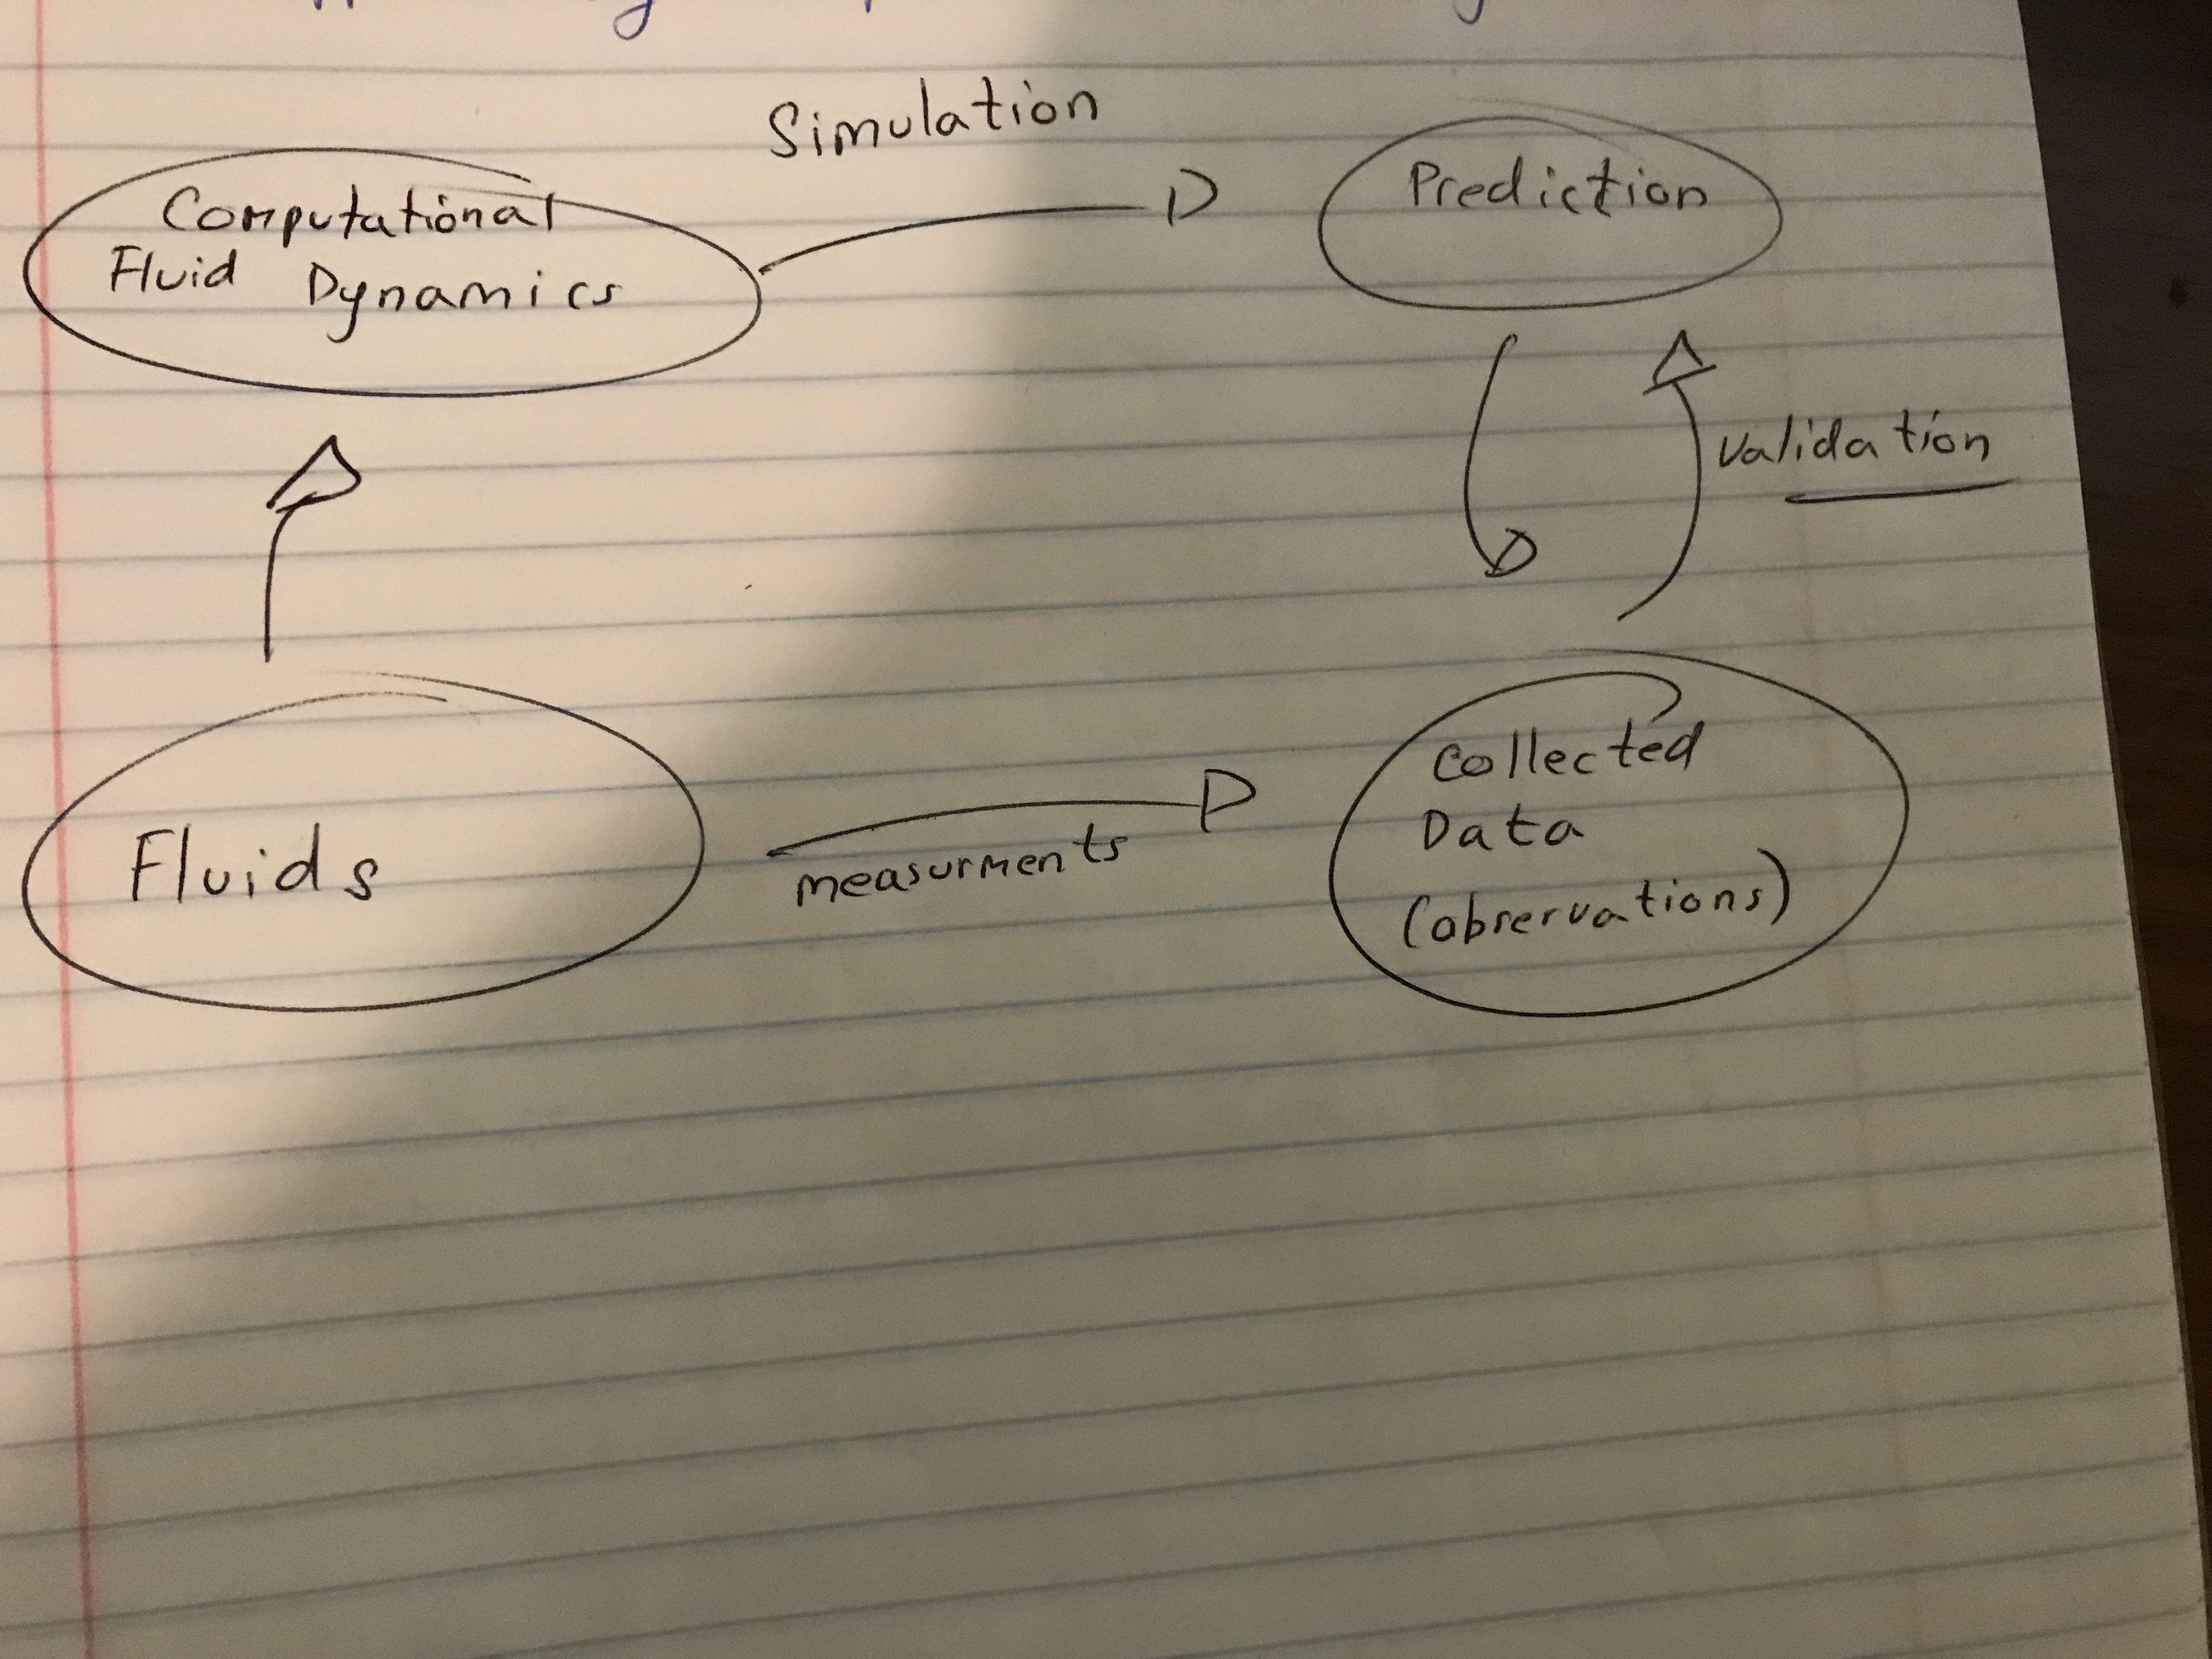
\includegraphics[width=.5\linewidth, height=.5\linewidth]{/Users/bryanlliguicota/Documents/Math_390.4_Data_Science_via_Machine_learning/hw01/IMG_0105.jpg}
  \label{fig:boat1}
\end{figure}


\easysubproblem{Pursuant to the fix in the previous question, how do we define \emph{data} for the purposes of this class?}\spc{3}
\\Data is what the reality "the world" gives us, we use it as a reference point for our predictions. The output data from our model will be compared to the data given to use from reality so we may measure its accuracy.
\easysubproblem{Pursuant to the fix in the previous question, how do we define \emph{predictions} for the purposes of this class?}\spc{3}
\\perdictions are what we obtain from our model when we input our data set $\mathbb{D}$. These predictions may or may not match the true outputs. That's where your measurements come into play to see how far you strayed away from the true output.
\easysubproblem{Why are \qu{all models wrong}? We are quoting the famous statisticians George Box and Norman Draper here.}\spc{2}
\\All models are wrong, because we can never know the true casual inputs. Their will always be an error due in ignorance in out algorithms and  independent variables, as well estimation error and misspecification error.
\intermediatesubproblem{Why are \qu{[some models] useful}? We are quoting the famous statisticians George Box and Norman Draper here.}\spc{2}
\\some models are useful b/c they fit to a acceptable degree the real world data we collected. In other words the data obtained from out model is close enough to the data from the real world.
\easysubproblem{What is the difference between a "good model" and a "bad model"?}\spc{2}
\\ The difference from a "good model" and "bad model", is basically how close our $y_{i}$ is from  $\hat{y_{i}}$. This can be due many factors such as out data set $\mathbb{D}$ and out chooses from the input space $\mathcal{X}$, they may stray away to much from the true causal inputs $\mathcal{Z}$
\end{enumerate}

\problem{We are now going to investigate the aphorism \qu{An apple a day keeps the doctor away}. We will use this as springboard to ask more questions about the framework of modeling we introduced in this class.}

\begin{enumerate}

\intermediatesubproblem{How good / bad do you think this model is and why?}\spc{3}
\\This is a bad model because our set of independent variables are stray to much from the true casual inputs.
\easysubproblem{Is this a mathematical model? Yes / no and why.}\spc{3}
\\Yes it can be turned into a mathematical model based on how we give a numeric value to the outcome and inputs.
\easysubproblem{What is(are) the input(s) in this model?}\spc{3}
\\In the model the inputs are the consumption of apples in a day, or average in a range of days.
\easysubproblem{What is(are) the output(s) in this model?}\spc{3}
\\The output is whether or nor the person is healthy. How we will measure "health" is something else. 
\easysubproblem{Devise a means to measure the main input. Call this $x_1$ going forward.}\spc{4}
\\Based on a range of days, lets say 5 on average how many apples did the individual eat.
\easysubproblem{Devise a means to measure the main output. Call this $y$ going forward.}\spc{4}
\\The persons health, based on whether or not he/she saw the doctor.
\easysubproblem{What is $\mathcal{Y}$ mathematically?}\spc{3}
\\1 - has not seen the doctor
\\0- has seen the doctor
\easysubproblem{Briefly describe $z_1, \ldots, z_t$ in English where $y = t(z_1, \ldots, z_t)$ in this \emph{phenomenon} (not \emph{model}).}\spc{3}
\\$z_1, \ldots, z_t$ are the true casual inputs, ant $t$ is the true relation function b/w the  true inputs and outputs.
\easysubproblem{From this point on, you only observe $x_1$ is in the model. What is $p$ mathematically?}\spc{1}
\\$p$ represents the dimension we are working in. Since we only observe one independent variable $x_1$, our $p$ is only one. $$x_1 \in \mathbb{R}^{p = 1}$$

\intermediatesubproblem{From this point on, you only observe $x_1$ is in the model. What is $\mathcal{X}$ mathematically? If your information contained in $x_1$ is non-numeric, you must coerce it to be numeric at this point.}\spc{3}
\\$\mathcal{X}$ is our input space, a countable infinity set of independent variables, some of which we can observe. $$x_{1} \in \mathcal{X}$$ Because we are dealing with mathematical models if $x_{1}$ is not numeric, it will have to be altered. This is where bias may come into play, if $x_1$ is categorical suppose $n$ categories, than we can associate each category with a number ${1}...{n}$. This has its downside, b/c we may be giving one category more importance than the other.
\intermediatesubproblem{How did we term the functional relationship between $y$ and $x_1$?}\spc{3}
\begin{eqnarray*}
y&\approx& f(x_{1})\\
y&=&f(x_{1})+\delta  \\
\text{where } \delta &\equiv& t(z_{1}) - f(x_{1}) \text{ is error due to ignorance}\\
\end{eqnarray*}
\easysubproblem{Briefly describe \emph{superivised learning}.}\spc{5}
\\Supervised learning is a method used to train our learning algorithm. We are given historical data and the true causal output for a set of $x$ in the data. We use this data to alter out weights to obtain an optimal solution.
\easysubproblem{Why is \emph{superivised learning} a \emph{empirical solution} and not an \emph{analytic solution}?}\spc{3}
\\supervised learning is an empirical solution b/c we going through many iterations to obtain an output based on a dataset. The output is gained through "observations/experiences", while a  analytical solution involves proofs and a series of logical steps. 
\intermediatesubproblem{From this point on, assume we are involved in supervised learning to achieve the goal you stated in the previous question. Briefly describe what $\mathbb{D}$ would look like here.}\spc{3}
\\$\mathbb{D}$ is composed of the training data, if we are only observing one independent variable $x_1$ we can have it be whether or not they had an apple, or how many apples they consumed on average during a given time period. Each $y$ associated with an $x_1$ could be the persons health. There are many ways to measure a persons health, one could be the number of times he/she went to the doctor in the time frame specified above. 
\intermediatesubproblem{Briefly describe the role of $\mathcal{H}, \mathcal{A}$ here.}\spc{3}
\\$\mathcal{H}$ is the set of candidate functions, because we are dealing with only one variable I think it should be composed of threshold parameters. Maybe eating a certain amount of apple a day for a given period on average really does keep you healthy. If that's the case, what we want to know is what is that range. To much of something is bad and so is to little, finding the sweet spot would mean have 2 threshold values to indicate your range.
\\$\mathcal{A}$ is the algorithm we use to find an optimal function given $\mathbb{D}$ and $\mathcal{H}$
\easysubproblem{If $g = \mathcal{A}(\mathbb{D}, \mathcal{H})$, what should the domain and range of $g$ be?}\spc{3}
\\Based on my response to the previous question, the domain  $(\mathbb{D}, \mathcal{H})$ would be the training data and set of candidate functions. The range would be a tuple of two values indicating a low and high for  the number of acceptable apples one can eat and be healthy(say away from the doctor as much as possible).
\easysubproblem{Is $g \in \mathcal{H}$? Why or why not?}\spc{3}
\\ Yes,  $g \in \mathcal{H}$. This doe not necessarily mean that we choose the best candidate function. The best possible function in $\mathcal{H}$ is   $h^{\star}$, but it is unlikely we choose it.
\easysubproblem{Given a never-before-seen value of $x_1$ which we denote $x^*$, what formula would we use to predict the corresponding value of the output? Denote this prediction $\hat{y}^*$.}\spc{3}
$$\hat{y}^* = g(x^*)$$
\intermediatesubproblem{Is it reasonable to assume $f \in \mathcal{H}$? Why or why not?}\spc{4}
\\No it not reasonable to assume $f \in \mathcal{H}$ since this would mean that we obtain the best possible function that approximates the real world. What is reasonable to assume is the $h^* \in \mathcal{H}$, where $h^*$ is the best approximation of  $f \in \mathcal{H}$.
\easysubproblem{If $f \notin \mathcal{H}$, what are the three sources of error? Write their names and provide a sentence explanation of each. Note that I made a notational mistake in the notes based on what is canonical in data science. The difference $t - g$ should be termed $e$ as the term $\mathcal{E}$ is reserved for $t - h^*$.}\spc{4}
\\When $f \notin \mathcal{H}$ the three possible errors are:
\\$ 1.\text{ } (t(\vec{z}) - f(\vec{x}))$ Denoted as error due to ignorance. This error will always exist, and the best we can do is try to minimize it. It represents the difference b/w the true relation function $t$ and the best approximation function $f$.
\\$ 2.\text{ } ( f(\vec{x})- h^*(\vec{x}))$ Denoted as the misspecification error; this is the difference b/w out best approximation of the real world function $f$ and the best candidate function $ h^* \in \mathcal{H}$. 
\\$ 3.\text{ } ( h^*(\vec{x})- g(\vec{x}))$ Denoted as the estimation error, it says that even if the best candidate function is our set, their is still a good chance that we may not even pick it. Instead the candidate function we end up with is $g$. The estimation error is their to tell us how far we are from the best candidate function $h^*$.
\intermediatesubproblem{For each of the three source of error, provide a means of reducing the error. We discussed this in class.}\spc{4}
\\- For error 1 (error due to ignorance) we can improve it by increasing the amount of data we have and improving or independent variables we choose from the input space.
\\- For error 2(misspecification error) This can be improved by increasing our set of candidate functions, as well as improving our algorithm.
\\- For error 3(estimation error) this error can be decreased by improving out algorithm $\mathcal{A}$
\easysubproblem{Regardless of your answer to what $\mathcal{Y}$ was above, we now coerce $\mathcal{Y} = \braces{0,1}$. If we use a threshold model, what would $\mathcal{H}$ be? What would the parameter(s) be?}\spc{3}
\\Demote the threshold as b:
\begin{eqnarray*}\\
\hat y_{i}=1 \ iff   x_{i}  \geq b \\
\hat y_{i}=0  \ iff   x_{i}  < b \\
\end{eqnarray*}
We would have $\mathcal{H} = \{ \mathbbm{1}_{ \vec{w}\cdot \vec{x}  \geq b}  :  x\in \mathbb{R} \land w\in \mathbb{R} \}$
\easysubproblem{Give an explicit example of $g$ under the threshold model.}\spc{3}
\\Lets say the best number of apples to eat in 5 days is 7. On average people who ate more than seven apples in the course of five days lived healthier than those who didn't. Therefore out threshold is 7, anything 7 or greater will be classified as $1$, anything less than $7$ will be a 0.  Now if we introduce a person who has eaten 100 apples in 5 days (with an average of 20 per day) we will classify him/her as a 1 (healthy).
\end{enumerate}

\problem{These are questions about the linear perceptron. This problem is not related to problem 3.}

\begin{enumerate}

\easysubproblem{For the linear perceptron model and the linear support vector machine model, what is $\mathcal{H}$? Use $b$ as the bias term.}\spc{3}
\\
In both the linear perceptron model and the linear support vector machine $\mathcal{H}$ is considered the set ("pool") of candidate functions (linear classifiers) .For the perceptron model $ \mathcal{H}$ is the set of indicator functions which give out a binary response of 0 or 1 based on the dot product of the weight vector $\vec{w}$ and independant variable $\vec{x}$ (the bias $b$ is $w_{0}$ in the weight matrix). For the support vector machine $\mathcal{H}$ consists of linear functions that meet the condition  $\forall_i$ $(y_i-\frac{1}{2})(\vec{w}\cdot\vec{x}_{i} + b)\geq \frac{1}{2}$
\intermediatesubproblem{Rewrite the steps of the \emph{perceptron learning algorithm} using $b$ as the bias term.}\spc{13}
\\Let $\mathcal{X} = \mathbb{R}^d$ be the input space, where $d$ represents the dimension we are working in. The space $\mathcal{Y} = \{ 1,0\}$, is the output space denoted by a binary decision. $x_{1 \cdot}, \ldots, x_{d\cdot} \in \mathbb{R}^d $ correspond to features in our supervised learning algorithm(the perceptron).We will  have a hypothesis set of candidate functions $\mathcal{H}$, as well as weights $w_{1 \cdot}, \ldots, w_{d\cdot} \in \vec{w}$.  Our threshold is another factor that is taken into account, the threshold is denoted as $b$ (bias). 
\begin{eqnarray*}\\
\hat y_{i}=1 \ iff  \sum_{i=1}^{d}  w_{i} \cdot x_{i}  > b \\
\hat y_{i}=0  \ iff  \sum_{i=1}^{d}  w_{i} \cdot x_{i}  < b \\
\end{eqnarray*}
The bias can show how lenient to strict the model is. The perceptrons learning algorithm $\mathcal{A}$ will search $\mathcal{H}$ for weights and bias that perform well on the data set. The optimal weights and bias define the final hypothesis $g \in \mathcal{H} $ . Suppose we are working in a 2 dimensional space, our parameters $w_{1}, w_{2}, b$ correspond to different lines $w_{1}x_{1} + w_{2}x_{2} + b= 0$. We can simplify the notation of the perceptron formula by letting the bias $b$ be the weight $w_{0} = b$, we will need to increment the number of elements in $\vec{x}$ in order to do the dot product, let $x_{0} = 1$. With all the notation done we now move to the perceptron learning algorithm PLA. The PLA determines $\vec{w}$ based on historical data we provide it with $\mathbb{D}$.  Assuming the data is linear separable, we use a simple iterative method to determine the optimal $\vec{w}$. During the $i_{th}$ iterative step the current weight vector is $w_{i}$. The algorithm picks a point from $\mathbb{D}$ lets say $(x_{i} , y_{i})$ and uses it to output a $\hat{y_{i}}$ that is compared to $y_i$,based on the difference $w_{i+1}$ is modified.
$$w_{i+1} = w_{i}+(\hat{y_{i}}- y_{i})x_{i}$$
\easysubproblem{Illustrate the perceptron as a one-layer neural network with the Heaviside / binary step / indicator function activation function.}\spc{10}
\\A threshold determines if a neuron fires. A threshold is a type of activation function,  an activation function determines the range of values that will cause the neurons to fire. The threshold is a simple activation function, in our case an indicator function  will be used as a activation function that fires either a 0 or a 1 based on input values.
\begin{figure}[h!]
  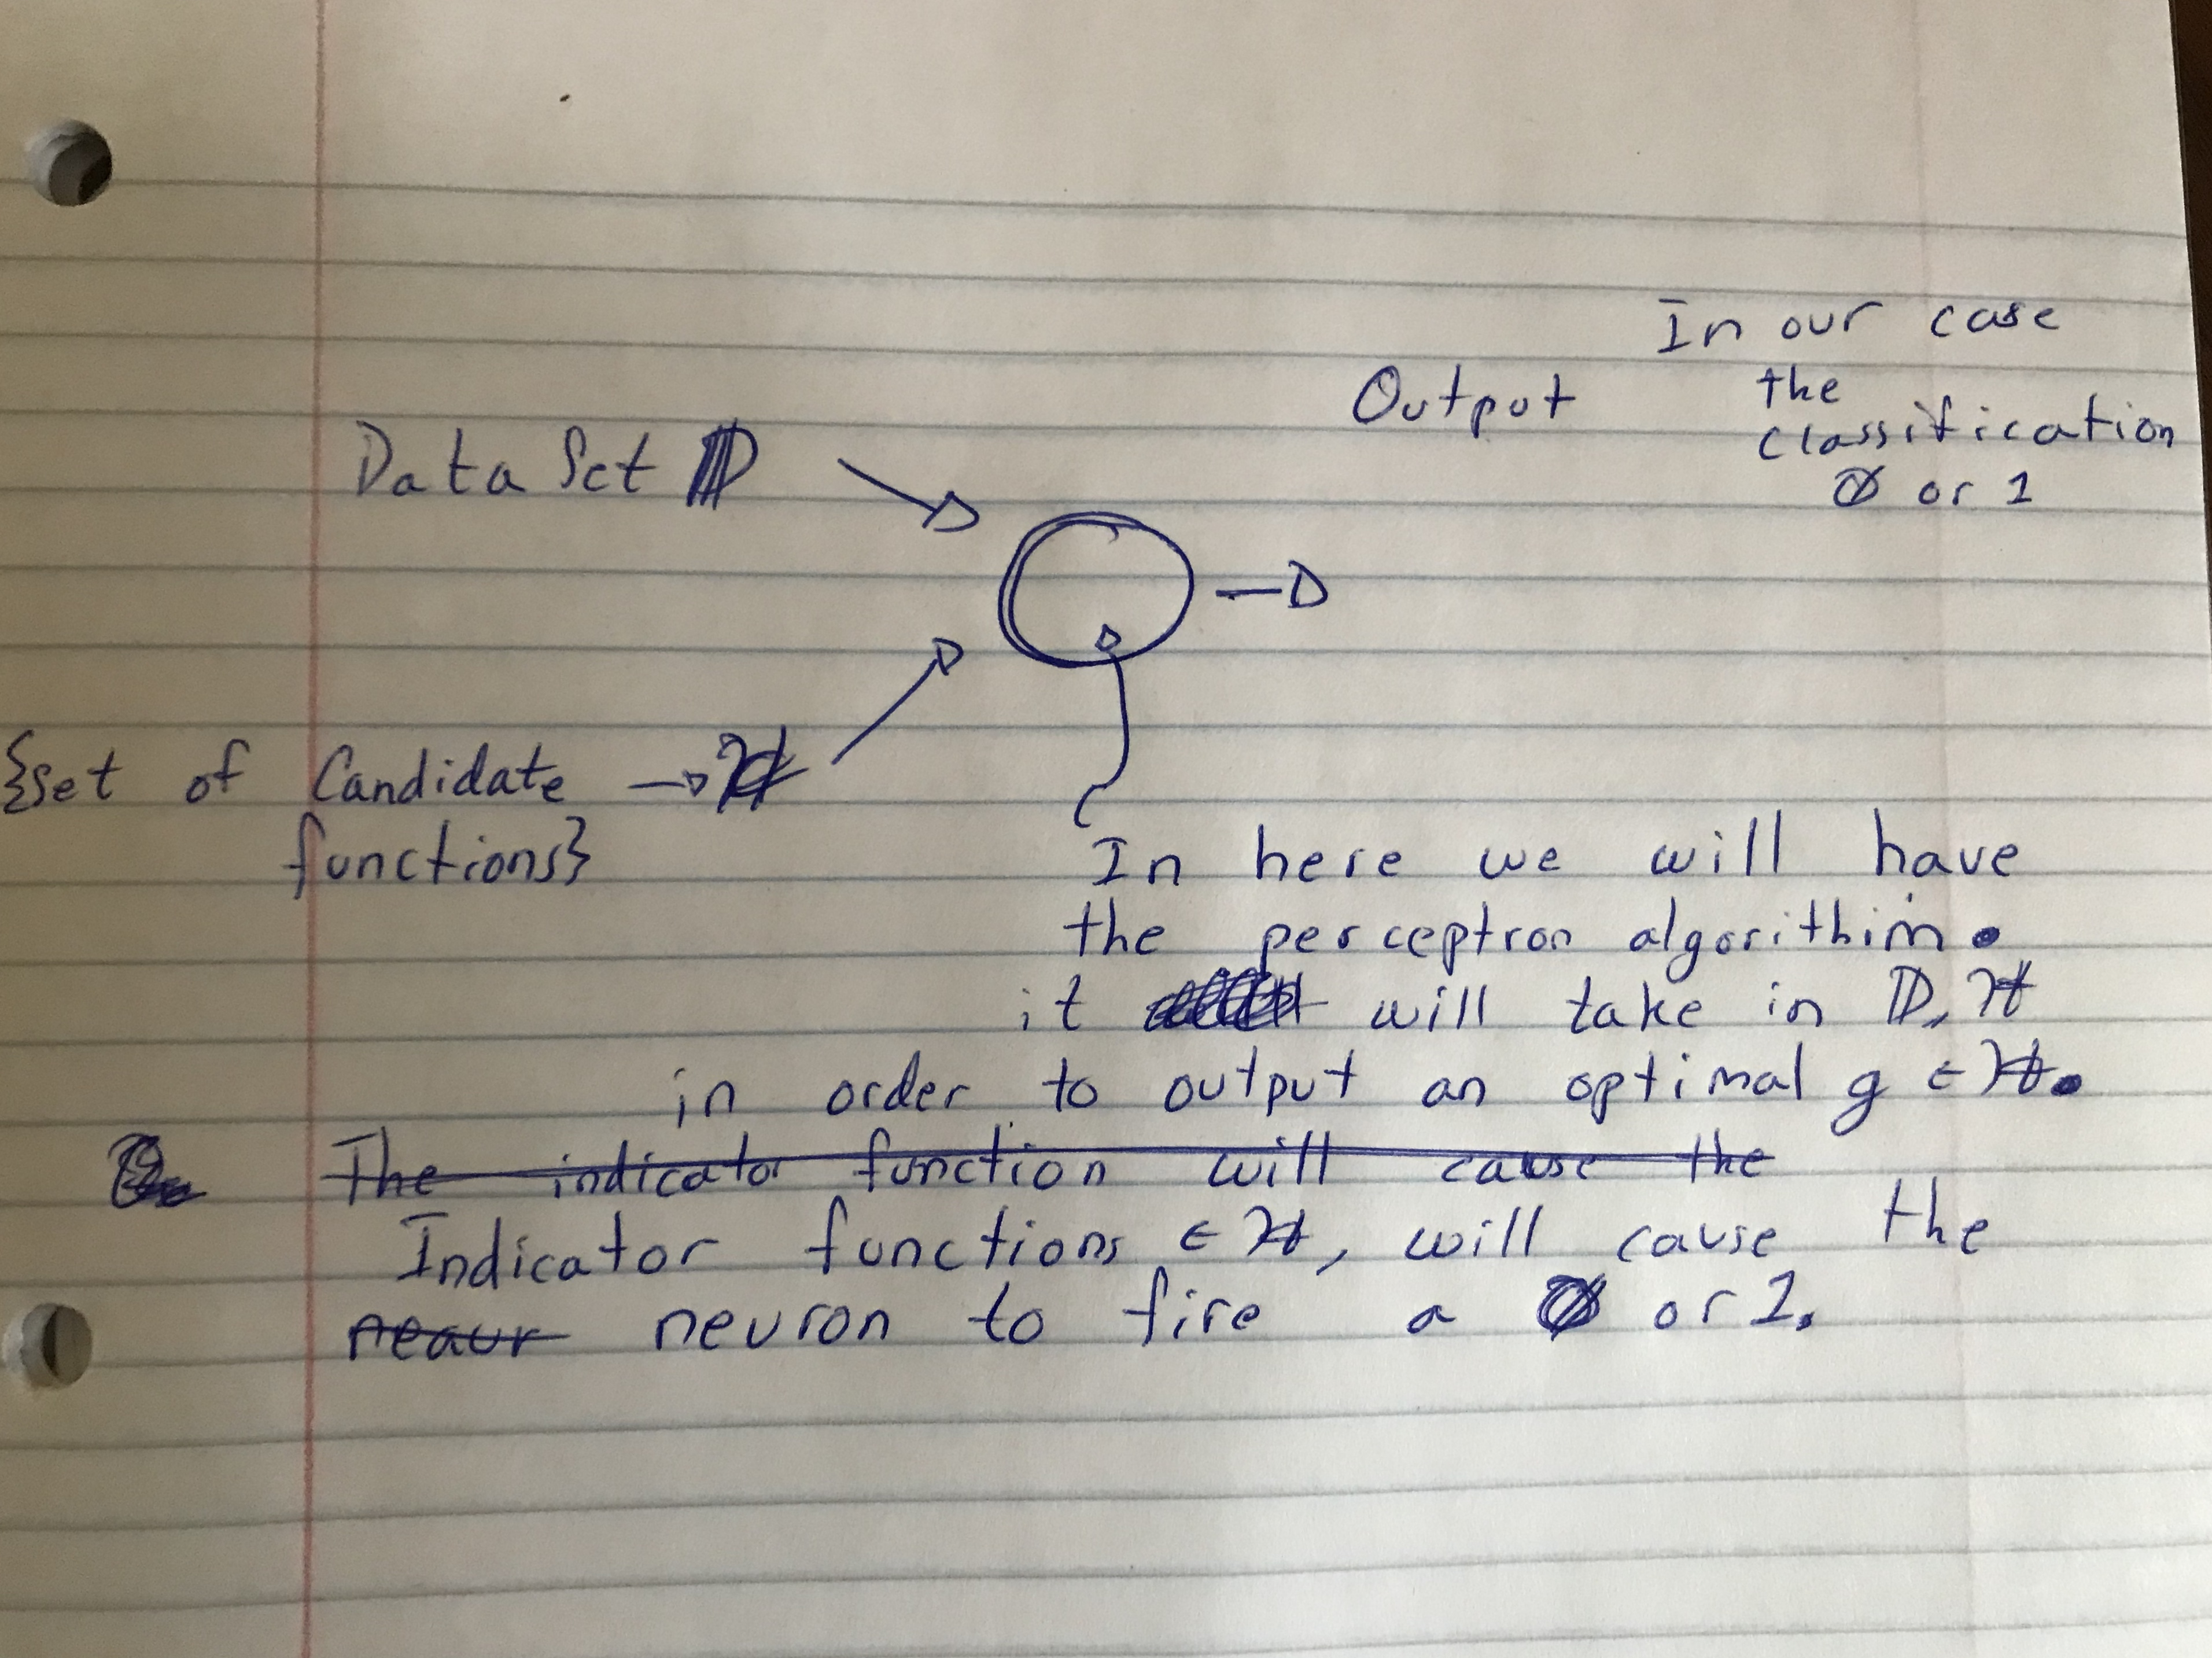
\includegraphics[width=.5\linewidth, height=.5\linewidth]{/Users/bryanlliguicota/Documents/Math_390.4_Data_Science_via_Machine_learning/hw01/IMG_0103.jpg}
  \caption{1 layered N.N.}
  \label{fig:boat1}
\end{figure}


\easysubproblem{Provide an illustration of a two-layer neural network. Be careful to indicate all pieces. If a mathematical object has a different value from another mathematical object, denote it differently.}\spc{10}
\begin{figure}[h!]
  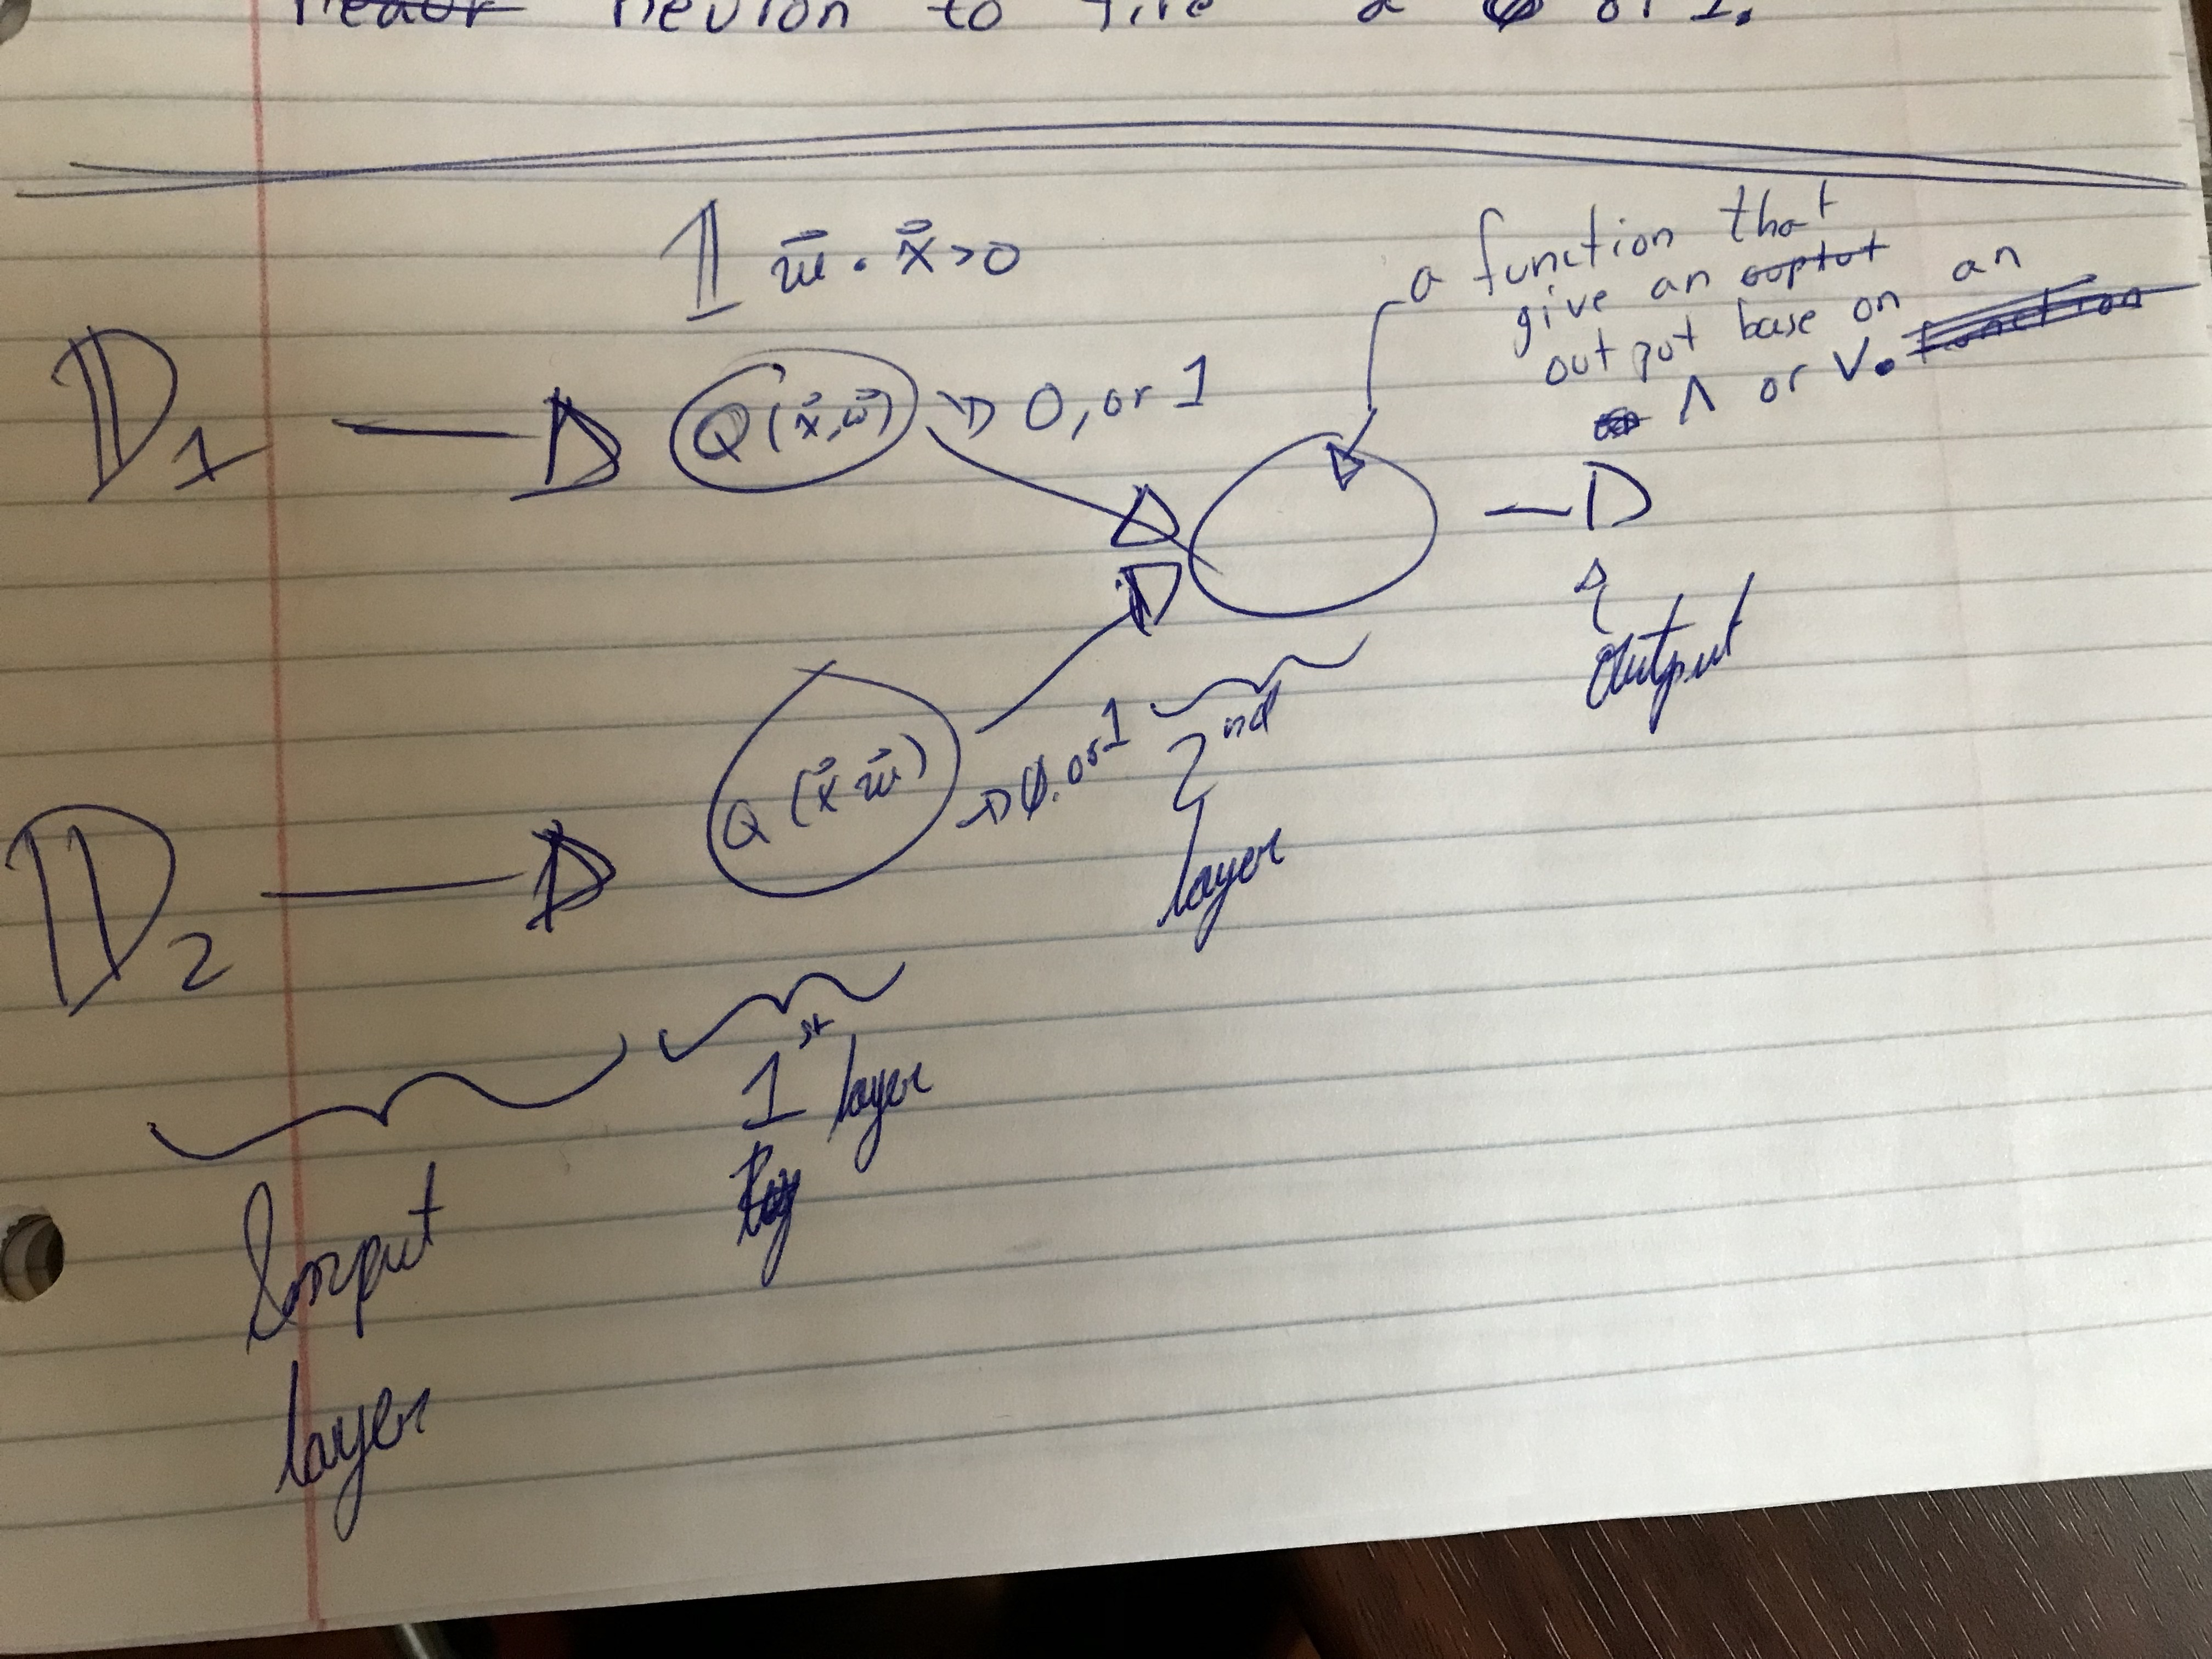
\includegraphics[width=.4\linewidth, height=.4\linewidth]{/Users/bryanlliguicota/Documents/Math_390.4_Data_Science_via_Machine_learning/hw01/IMG_0104.jpg}
  \caption{2 layered N.N.}
  \label{fig:boat1}
\end{figure}
\end{enumerate}

\end{document}

